\section{Introduction}


%Repeat what was in the intro a bit

%Why do this?

%say something about \texttt{mmds}

%Do I need to say something about Len here?

% talk about the R package here

\section{General formulation}

This section lays out a mixture model formulation for distance sampling detection functions. Beginning with the simplest case (line transects with no covariates) the models are built up and it is shown that the simpler models are just special cases of the more complex ones, thus providing a general framework for mixture model detection functions.

The core principle here is to replace the ``key function plus adjustment terms'' model for the detection function with a mixture model. The simplest example would be to define the detection function, $g$, as some finite weighted sum of half-Normal distributions:
\begin{equation}
g(x;\bm{\sigma},\bm{\pi}) = \sum_{j=1}^J \pi_j \exp \Big( \frac{-x^2}{2 \sigma_j^2}\Big).
\label{mmds-simplemix}
\end{equation}
Where the mixture proportions, $\pi_j$, have the property $\sum_{\forall j}\pi_j=1$ and $\bm{\pi} = (\pi_1, \dots, \pi_J)$. $\bm{\sigma}=(\sigma_1,\sigma_2,\dots,\sigma_J)$ are scale parameters. An example of a 2-point mixture of half-Normals is given in figure \ref{2ptdia}.

TKTKTK physical explanation of models - interpretation as smooths curves vs. interpretation as sub-populations.

\begin{figure}
\centering
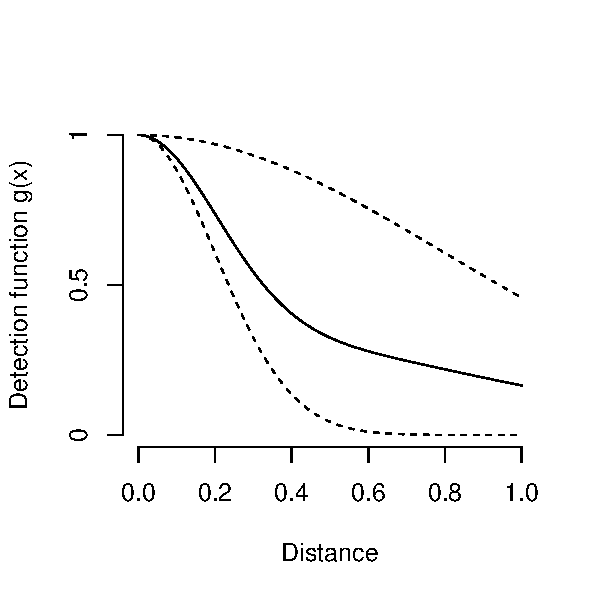
\includegraphics[width=3in]{mix/figs/2ptdia.pdf}
\caption{An example of a 2-point mixture of half-Normals. The two constituent mixture components are shown with dashed lines, the whole mixture function is the solid line. The scale parameters are $0.8$ and $0.2$. The associated mixture proportions are $0.64$ and $0.36$.}
\label{2ptdia}
\end{figure}

Clearly one can think of many variations on this theme: alternative functions, different functions for each mixture component, continuous mixtures or a finite mixture of continuous and finite mixtures (\textit{a la} \cite{morgan08}). However, here only finite mixtures of half-Normals are considered.

\subsection{Line transects}
For line transects, we can simply substitute equation (\ref{mmds-simplemix}) into the line transect likelihood in equation (\ref{ds-lt-likelihood}). Before doing this we first note that the definition of $\mu$ has not changed, merely the definition of $g$. Denoting $g_j$ as one of the component detection functions of the mixture,
\begin{align*}
\mu = \int_0^w \sum_{j=1}^J \pi_j g_j(x;\sigma_j) \text{d}x = \sum_{j=1}^J \pi_j \int_0^w  g_j(x;\sigma_j) \text{d}x = \sum_{j=1}^J \pi_j \mu_j.
\end{align*}
So, the likelihood is:
\begin{align}
\mathcal{L}(\bm{\sigma}, \bm{\pi}; \bm{x}) &= \prod_{i=1}^n f(x_i;\bm{\sigma}, \bm{\pi}),\\
&= \prod_{i=1}^n \frac{g(x_i;\bm{\sigma}, \bm{\pi})}{\mu},\\
&= \prod_{i=1}^n \frac{\sum_{j=1}^J \pi_j g_j(x_i;\sigma_j)}{\sum_{j=1}^J \pi_j \int_0^w  g_j(x;\sigma_j) \text{d}x},\\
&= \prod_{i=1}^n \sum_{j=1}^J \pi_j \frac{\exp \Big( \frac{-x_i^2}{2 \sigma_j^2}\Big)}{\int_0^w \exp \Big( \frac{-x_i^2}{2 \sigma_j^2}\Big) \text{d}x}.
\label{mmds-lt-likelihood}
\end{align}


Rather than decomposing $g$ into its constituent $g_j$s, the likelihood can be thought of as a mixture of PDF components, $f_j$, yielding the same final expression:
\begin{align}
\mathcal{L}(\bm{\sigma}, \bm{\pi}; \bm{x}) &= \prod_{i=1}^n f(x_i;\bm{\sigma}, \bm{\pi}),\\
&= \prod_{i=1}^n \sum_{j=1}^J \pi_j f_j(x_i;\bm{\sigma}, \bm{\pi}),\\
&= \prod_{i=1}^n \sum_{j=1}^J \pi_j \frac{\exp \Big( \frac{-x_i^2}{2 \sigma_j^2}\Big)}{\int_0^w  \exp \Big( \frac{-x_i^2}{2 \sigma_j^2}\Big) \text{d}x}.
\label{mmds-lt-likelihood-pdf}
\end{align}

\subsection{Point transects}
The detection function is, of course, the same for point transects as for line transects. What changes is the PDF and hence likelihood. The likelihood is therefore:
\begin{align}
\mathcal{L}(\bm{\sigma}, \bm{\pi}; \bm{r}) &= \prod_{i=1}^n f(r_i;\bm{\sigma}, \bm{\pi}),\\
&= \prod_{i=1}^n \sum_{j=1}^J \pi_j f_j(r_i; \sigma_j),\\
&= \prod_{i=1}^n \sum_{j=1}^J \pi_j \frac{g_j(r_i; \sigma_j,)}{\nu_j},\\
&= \prod_{i=1}^n \sum_{j=1}^J \pi_j \frac{r_i \exp \Big( \frac{-r_i^2}{2 \sigma_j^2}\Big)}{\int_0^w r  \exp \Big( \frac{-r_i^2}{2 \sigma_j^2}\Big) \text{d}r}.
\label{mmds-pt-likelihood-pdf}
\end{align}
where we can define a per-mixture effective area of detection:
\begin{equation}
\nu_j= 2 \pi \int_0^w r  g_j(r;\sigma_j) \text{d}r,
\end{equation}
which is analogous to $\mu_j$, above, and an overall area of detection:
\begin{equation}
\nu= \sum_{j=1}^J \pi_j \nu_j.
\end{equation}


Having these two likelihoods written down, the formulation for covariate models and the generalised likelihood can be derived.

\subsection{Covariate models}
The above models show that the differences between the CDS and mixture model DS (MMDS) are fairly minimal. For the covariate case things are a little more tricky. There are many possible model formulations and the notation is therefore more complicated.

Consider the case where one distance, $x$ (alternatively $r$ for point transects), has been observed and a set of corresponding covariates $z_1,\dots,z_K$ have been recorded too. As in MCDS the scale function is thought of as a (link) function of these covariates and a set of coefficients, the detection function is then defined as:
\begin{equation*}
g(x, \bm{z};\bm{\beta},\bm{\pi}) = \sum_{j=1}^J \pi_j \exp \Big( \frac{-x^2}{2 \sigma_j(\bm{z};\bm{\beta}_j)^2}\Big),
\label{mmds-detfct-covar}
\end{equation*}
and the scale parameter per mixture is defined as:
\begin{equation*}
\sigma_j(\bm{z};\bm{\beta}_j) = \exp \Big(\beta_{0j} + \sum_{k\in K_j} \beta_{kj} z_k \Big),
\end{equation*}
where $\bm{z}$ is the $K$-vector of all covariates. $K_j$ is the set of covariates to be used with mixture $j$. The vector of per mixture coefficients is $\bm{\beta}_j=(\beta_{0j},\{ \beta_{kj} : k \in K_j\})$. Finally $\bm{\beta}=(\bm{\beta}_1,\dots,\bm{\beta}_J)$ is the vector of all coefficients ordered by mixture part then covariate.

When we have multiple observations we store the distances in $\bm{x}$ (an $n$-vector). Then, for each observation we have a $\bm{z}_i$, which is a vector of covariates for that particular observation. $Z$ is an $n \cross K$ matrix of all covariates ie. the $\bm{z}_i$s stacked on top of each other. So then $z_{ik}$ would be the $i^\text{th}$ observation's covariate $k$ (and the $ik^\text{th}$ element of $Z$).

TKTKTK more here

%\subsubsection{Covariates - intercept model}
%
%One can think of a special case of the model above when the parameters estimated are common across all mixture components, except for an intercept.  Mathematically,
%\begin{align*}
%\sigma_j(\bm{z};\bm{\beta}_j) = \exp \Big(\beta_{0j} + \sum_{k\in K_j} \beta_{k} z_k \Big)
%\end{align*}
%so the $\beta_{0j}$s are estimated in each mixture but the $\beta_{k}$s are common to all mixtures and are estimated simultaneously. In this case, the $K_j$s are the same for all mixture components.
%
%NOT CURRENTLY IMPLEMENTED

\subsection{Generalised likelihood}
\label{ds-genlik}

\subsubsection{Line transects}
Considering the non-covariate case as a special case of the covariate model, the likelihood can then be written as:
\begin{align}
\mathcal{L}(\bm{\beta}, \bm{\pi} ; \bm{x}, Z) &= \prod_{i=1}^n f(x_i;\bm{\sigma}(\bm{z}_i, \bm{\beta})),\\
&= \prod_{i=1}^n \frac{g(x_i;\bm{\sigma}(\bm{z}_i, \bm{\beta}))}{\mu(\bm{z}_i)},\\
&= \prod_{i=1}^n \sum_{j=1}^J \pi_j \frac{g_j(x_i; \sigma_j(\bm{z}_i;\bm{\beta}_j))}{ \mu_j(\bm{z}_i)}.
\label{mmds-lt-glikelihood}
\end{align}
where $\mu(\bm{z}_i)$ is the sum of the $\mu_j$s per observation, i.e.
\begin{equation}
\mu(\bm{z}_i) = \sum_{j=1}^J \pi_j \int_0^w g_j(x; \sigma_j(\bm{z}_i;\bm{\beta}_j)) \text{d}x.
\end{equation}
where the $\sigma_j(\bm{z}_i;\bm{\beta}_j)$s take the covariate form above; in the case of a no covariate model, there is only the intercept term, $\beta_{0j}$ ie:
\begin{equation}
\sigma_j = \exp ( \beta_{0j} ).
\end{equation}

\subsubsection{Point transects}
For point transects the likelihood is similar, though with the $r$ pre-multiplier as seen for CDS and MCDS:
\begin{align}
\mathcal{L}(\bm{\beta}, \bm{\pi} ; \bm{r}, Z) &= \prod_{i=1}^n f(r_i;\bm{\sigma}(\bm{z}_i, \bm{\beta})),\\
&= \prod_{i=1}^n \frac{g(r_i;\bm{\sigma}(\bm{z}_i, \bm{\beta}))}{\nu(\bm{z}_i)},\\
&= \prod_{i=1}^n \sum_{j=1}^J \pi_j \frac{g_j(r_i; \sigma_j(\bm{z}_i;\bm{\beta}_j))}{ \nu_j(\bm{z}_i)}.
\label{mmds-pt-glikelihood}
\end{align}
So,
\begin{equation}
\nu(\bm{z}_i) = 2 \pi \sum_{j=1}^J \pi_j \int_0^w r g_j(r; \sigma_j(\bm{z}_i;\bm{\beta}_j)) \text{d}r.
\end{equation}


\subsection{Probability of detection}

(TKTKTK write more here!)

The detection probability, as we have seen, is a central concept in distance sampling. Notably, it can be used as a way of estimating abundance (via Horvitz-Thompson estimators). In this vein, the per-observation detectability is first derived. Next, an estimate of overall average detectability is often useful (and will be used later to asses the performance of the method), so this is also derived. Finally, the variance of the average detectability is also found and as a result of this, an estimator of the coefficient of variation is also given.

\subsubsection{Per-observation detectability}
When using covariates, each object effectively has its own detection function and hence its own per observation detectability. Calculating this is fairly simple. Starting from the definition of detectability given in equation (3.19) of Buckland \textit{et al} (2004) p 38 (modified slightly for notational consistency), the detection function is replaced with (\ref{mmds-detfct-covar}):
\begin{align*}
P_a(\bm{z}_i) =& \frac{\mu(\bm{z}_i)}{w},\\
=& \frac{1}{w} \int_0^w g(x; \sigma(\bm{z}_i,\bm{\beta})) \text{d}x,\\
=& \frac{1}{w} \int_0^w \sum_{j=1}^J \pi_j g_j(x; \sigma_j(\bm{z}_i, \bm{\beta}_j)) \text{d}x,\\
=& \frac{1}{w} \sum_{j=1}^J \pi_j \int_0^w  g_j(x; \sigma_j(\bm{z}_i, \bm{\beta}_j)) \text{d}x,
\end{align*}
so the detectability can now be calculated for each observation.


\subsubsection{Average detectability}
(TKTKTK  Fill this in!)

\subsubsection{Variance of $p$}

\subsubsection{CV}

\subsection{Goodness of fit testing}





%%%%%%%%%%%%%%%%%%%%%%%%%%%%%%%%%%%%%%%%%%%%%%%%%%%
\section{Implementation}
This section gives detail on the implementation of MMDS, particularly those used in the \textsf{R} package \texttt{mmds}.

(TKTKTK more here)

\subsection{Parametrisation of the scale parameters}
The parametrisation of the $\sigma_j$s given in section \ref{ds-genlik} is not only useful because it simplifies the notation in the likelihood. It also allows for unconstrained optimisation of the scale parameters in all situations. Since $\sigma_j$ must be positive, optimising a set of $\bm{\beta}_j$s on the log scale allows for the $\bm{\beta}_j$s to take values over all of $\mathbb{R}$.


\subsection{Parametrisation of the mixture proportions}
When using 2-point mixtures, the constraint that the $\pi_j$s must sum to unity is enforced by definition (since $\pi_2=1-\pi_1$). However, in $J$-point mixtures when $J>2$, ensuring that the proportions sum to 1 is not guaranteed. The obvious way to get around this would be to penalise the likelihood, should the optimisation procedure propose values for the $\pi_j$s that are not in accordance with this condition. This is, of course, inefficient and ugly. Instead, a parametrisation is used for the mixture proportions which yields $\pi_j$s that comply.

Rather than estimating the $\pi_j$s, estimate $\alpha_k$s, where the relationship between the two is:
\begin{equation*}
\pi_j = F(\sum_{k=1}^j e^{\alpha_k}) - F(\sum_{k=1}^{j-1} e^{\alpha_k}) \qquad \text{for } 1\leq j \leq J-1
\end{equation*}
and
\begin{equation*}
\pi_J = 1-\sum_{j=1}^{J-1} \pi_j
\end{equation*}
where $F$ is any continuous CDF on $(0,\infty]$. Exponentiation ensures that $e^{\alpha_j}\geq0$, so $\alpha_j$ may lie anywhere on $\mathbb{R}$ allowing unconstrained optimisation. Summing these orders the $\pi_j$s, since only offsets are estimated. Finally, using the cumulative density function ensures that the $\pi_j$s sum to $1$. In practise the $\text{Gamma}(3,2)$ CDF is (somewhat arbitrarily) used. Figure \ref{dlbpi} illustrates the relationship.

% illustration of the pi parametrisation - DLB's method
\begin{figure}
\centering
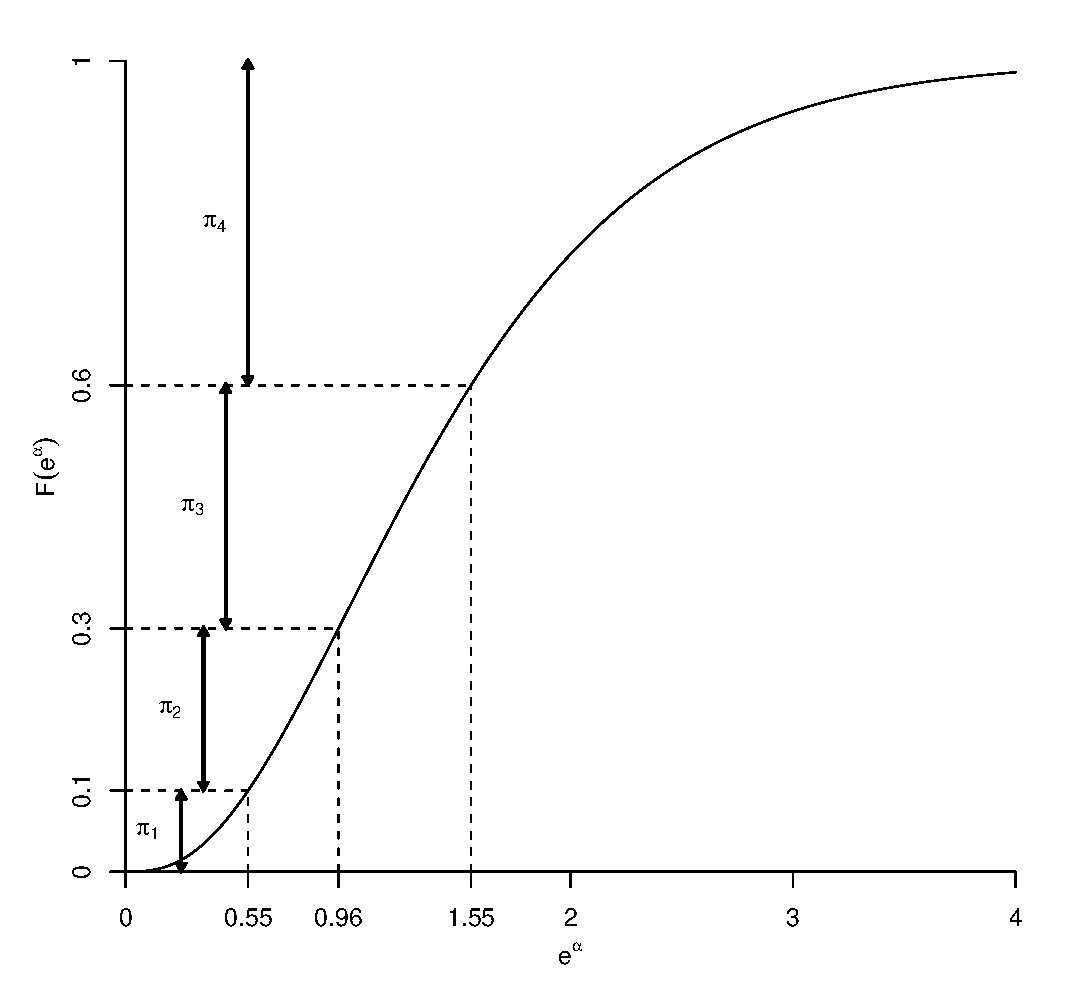
\includegraphics[width=4in]{mix/figs/pidia.pdf}
\caption{Illustration of the parameterisation of the $\pi_j$s. The black curve is a Gamma CDF (with shape parameter 3 and scale parameter 1/2). Here $\bm{\pi}=(0.1,0.2,0.3,0.4)$. The differences in the ``heights'' of the evaluations of the CDF give the values of $\pi_j$.}
\label{dlbpi}
\end{figure}

\subsubsection{Inverse transform}
\label{mmds-pi-inv}
To transform from the $\pi_j$s back to the $\alpha_j$s we simply re-arrange the above expression.
\begin{align*}
\pi_j &= F(\sum_{k=1}^j e^{\alpha_k}) - F(\sum_{k=1}^{j-1} e^{\alpha_k})\\
F(\sum_{k=1}^j e^{\alpha_k}) &= \pi_j + F(\sum_{k=1}^{j-1} e^{\alpha_k})\\
\sum_{k=1}^j e^{\alpha_k} &= F^{-1}(\pi_j + F(\sum_{k=1}^{j-1} e^{\alpha_k}))\\
e^{\alpha_j} &= F^{-1}\Big(\pi_j + F(\sum_{k=1}^{j-1} e^{\alpha_k})\Big) - \sum_{k=1}^{j-1} e^{\alpha_k}\\
\alpha_j &= \log_e \Big(F^{-1}\Big(\pi_j + F(\sum_{k=1}^{j-1} e^{\alpha_k})\Big) - \sum_{k=1}^{j-1} e^{\alpha_k}\Big)
\end{align*}
Thus, it is possible to move between $\pi_j$s and $\alpha_j$s easily.

\subsection{Fitting}
It is well known that mixture model likelihoods are notoriously multi-modal (\cite{BDA} PAGES).

(TKTKTK more here)

Three different strategies were used for the optimisation and offered in the \texttt{mmds} package. The justification being that if one method fails to fit a particular model, then perhaps another might be better at tackling that particular problem. The first and simplest of these methods is a straightforward quasi-Newton method, BFGS (\cite{bfgs}) which simply maximises the likelihood with the help of analytic gradients (see appendix \ref{appendix-mmds-derivs}). In testing this method was unsatisfactory so two other procedures were also developed.

\subsection{BFGS+SANN}
The starting value calculation (see section \ref{mmds-starting-vals}) is relatively primitive and therefore perhaps does not start the optimisation in a particularly good position to begin the maximisation. Given this and the rather complex likelihood, the odds are not stacked in the favour of the optimisation procedure being successful. In order to move around the parameter space, simulated annealing (\cite{numrec}, pp. 549--554) is used to begin the maximisation then followed by a BFGS round to find the maxima. Both BFGS and simulated annealing are available via the \texttt{optim()} function in the base \textsf{R} distribution.

In particular, simulated annealing is used for 250 iterations, then unconstrained BFGS after that. In an attempt to avoid local maxima, these two steps are looped for five iterations and the results stored. The model with the lowest AIC is then chosen from these. If no models fit in the first 5 iterations, the procedure continues until at least one model fits, or there have been 20 attempts at fitting, whichever comes first.

It is worth noting that the method may appear to fail to converge for all attempts, however this does not necessarily indicate that the model will never converge. The stochastic nature of simulated annealing means that it is entirely possible that further runs may yield a useful result.

\subsection{Expectation-Maximisation Algorithm}
A common (TKTKTK cite!) way of fitting mixture models is to use the Expectation-Maximisation (EM) algorithm of \cite{em}. (TKTKTK WHY?!)


\subsubsection{Overview}

(TKTKTK Re-write this)

Considering each of the observations as coming from one of the $J$ mixture components, we arrive at a latent variable interpretation of the mixture model. Given this latent variable view, it is possible to then evaluate the probability that each observation is from a particular mixture component. The mixture proportions can then we calculated by taking the expectation over the observations of these ``weights'' for a given mixture component. Once the mixture proportions are calculated, the scale parameters can be found using a some optimisation procedure (such as BFGS) keeping the mixture proportions constant within BFGS. This yields a new set of scale parameters, so the mixture proportions are then recalculated. EM switches between these two stages (expectation and maximisation) until the values for the mixture proportions and the scale parameters have converged.

\subsubsection{EM steps}
The expectation and maximisation steps are defined as follows. First note that $f_j(x_i;\sigma_j(\bm{z}_i,\bm{\beta}_j))$ is the PDF of mixture part $j$ evaluated at distance $x_i$ with covariates $\bm{z}_i$. 


\begin{itemize}
\item \textbf{Expectation.}
During the expectation step the mixture proportions are calculated. This is done using the expected values of the weights, $w_{ij}$, for each datum $i$ and mixture $j$,
\begin{equation*}
\mathbb{E}[w_{ij}] = \frac{\pi_j f_j(x_i;\sigma_j(\bm{z}_i,\bm{\beta}_j))}{\sum_{k=1}^J \pi_k f_k(x_i;\sigma_k(\bm{z}_i,\bm{\beta}_k))}.
\end{equation*}
Then $\pi_j$s may be calculated as:
\begin{equation*}
\pi_j=\frac{1}{n} \sum_{i=1}^n \mathbb{E}[w_{ij}].
\end{equation*}

\item \textbf{Maximisation.}
Keeping the $\pi_j$s fixed (from the previous step), optimise with respect to the $\sigma_j$s (or, rather, $\beta_{jk}$s). Here BFGS is used with analytic gradients (see appendix \ref{appendix-mmds-derivs}). 
\end{itemize}



cite EM/CEM/SEM paper

% maybe show why other parametrisation doesn't work??


\subsection{Starting values}
\label{mmds-starting-vals}
\cite{beavers98} give a method for estimating starting values for the scale parameter of a half-Normal detection function. In the non-covariate case, the estimate is given as the intercept parameter from intercept only regression on $\log(x+\frac{w}{1000})$ (where $w$ denotes the truncation distance, as above). For covariate models, the equation used for the $\sigma$ is used in the regression and the estimated parameters from the linear regression are used as the starting values for the $\beta$s.

A similar approach can be use in the mixture case by first sorting data by distance and then dividing it into $k$ equal parts (for a $k$ point mixture). For each of these parts a \cite{beavers98}-type estimate is used for the $\beta_{jk}$s (or $\beta_j$s in the non-covariate case).

For the $\alpha_j$s, a set of $\pi_j$ are generated as $1/k$ and then transformed by the procedure given in section \ref{mmds-pi-inv} to be on the $\alpha_j$ scale.


\subsection{Derivatives}

The derivatives needed for the optimisation procedures are derived in full in \appref{app-mixderivs}.

%%%%%%%%%%%%%%%%%%%%%%%%%%%%%%%%%%%%%%%%%%%%%%%%%%%
\section{Testing}

The models detailed above were run on both real and simulated data to test their efficacy. Simulations of the most common models are presented first, followed by analyses of real data. The analyses of real data are available as a vignette written in Sweave (\cite{sweave}) at URL HERE.

\subsection{Simulations}

Four classes of models were tested, giving a range of easy and hard problems over possible sampling scenarios. The classes were:
\begin{itemize}
	\item Non-covariate 2-point mixtures for line transect data.
	\item Non-covariate mixtures for point transect data.
	\item Non-covariate 3-point mixtures for line transect data.
	\item Covariate mixtures for line transect data.
\end{itemize}
In order to assess how well the models performed, two metrics were used. The first metric is parameter estimates returned from the optimisation procedure -- this should highlight that the optimisation is working numerically and can successfully recover the parameters. The second metric is the abundance estimate ($\hat{N}$). The latter measure may be important as changes in the parameters may give (approximately) equal values of $\hat{N}$, since the parameter estimates are not usually of interest (the ultimate output being the abundance or density estimate in a distance sampling analysis), it makes sense to look at $\hat{N}$.

For each set of parameters for each of the model classes, 500 realisations were generated at each of 5 sample sizes (30, 60, 120, 480, 960). The data generation process is given in detail in each section.

\subsubsection{Non-covariate 2-point mixtures for line transect data}

Five parameter combinations were used to test non-covariate 2-point mixtures the parameters are given in table \ref{mmds-nocov-simtable} (in the more human-readable $\sigma$ and $\pi$ parametrisation) and their corresponding detection functions are plotted in figure \ref{mmds-nocov-funcs}.

\begin{table}[ht]
\centering
\begin{tabular}{c c c c}
Sim no. & $\sigma_1$ & $\sigma_2$ & $\pi_1$\\
\hline
\hline
1 & 0.2 & 0.8 &  0.36\\
2 & 0.8 & 0.2 & 0.44\\
3 & 0.2 & 0.8 & 0.18\\
4 & 10  & 0.2 & 0.44\\
5 & 0.01&  0.8 & 0.29\\
\end{tabular}
\label{mmds-nocov-simtable}
\caption{Simulation parameters for the non-covariate simulations. (In $\sigma$ and $\pi$ parametrisation).}
\end{table}

The first three simulations give relatively simple scenarios with the same scale parameters but varying the mixture proportions, these check behaviour under ``easy'' conditions. The fourth checks to see what happens when one of the mixtures is essentially too big to be identified (it starts to decrease after the truncation distance so the parameter value could be 10, 100 or even 1000). Finally the fifth example gives and extremely spiked detection function.

% detection functions for nocov
\begin{figure}
\centering
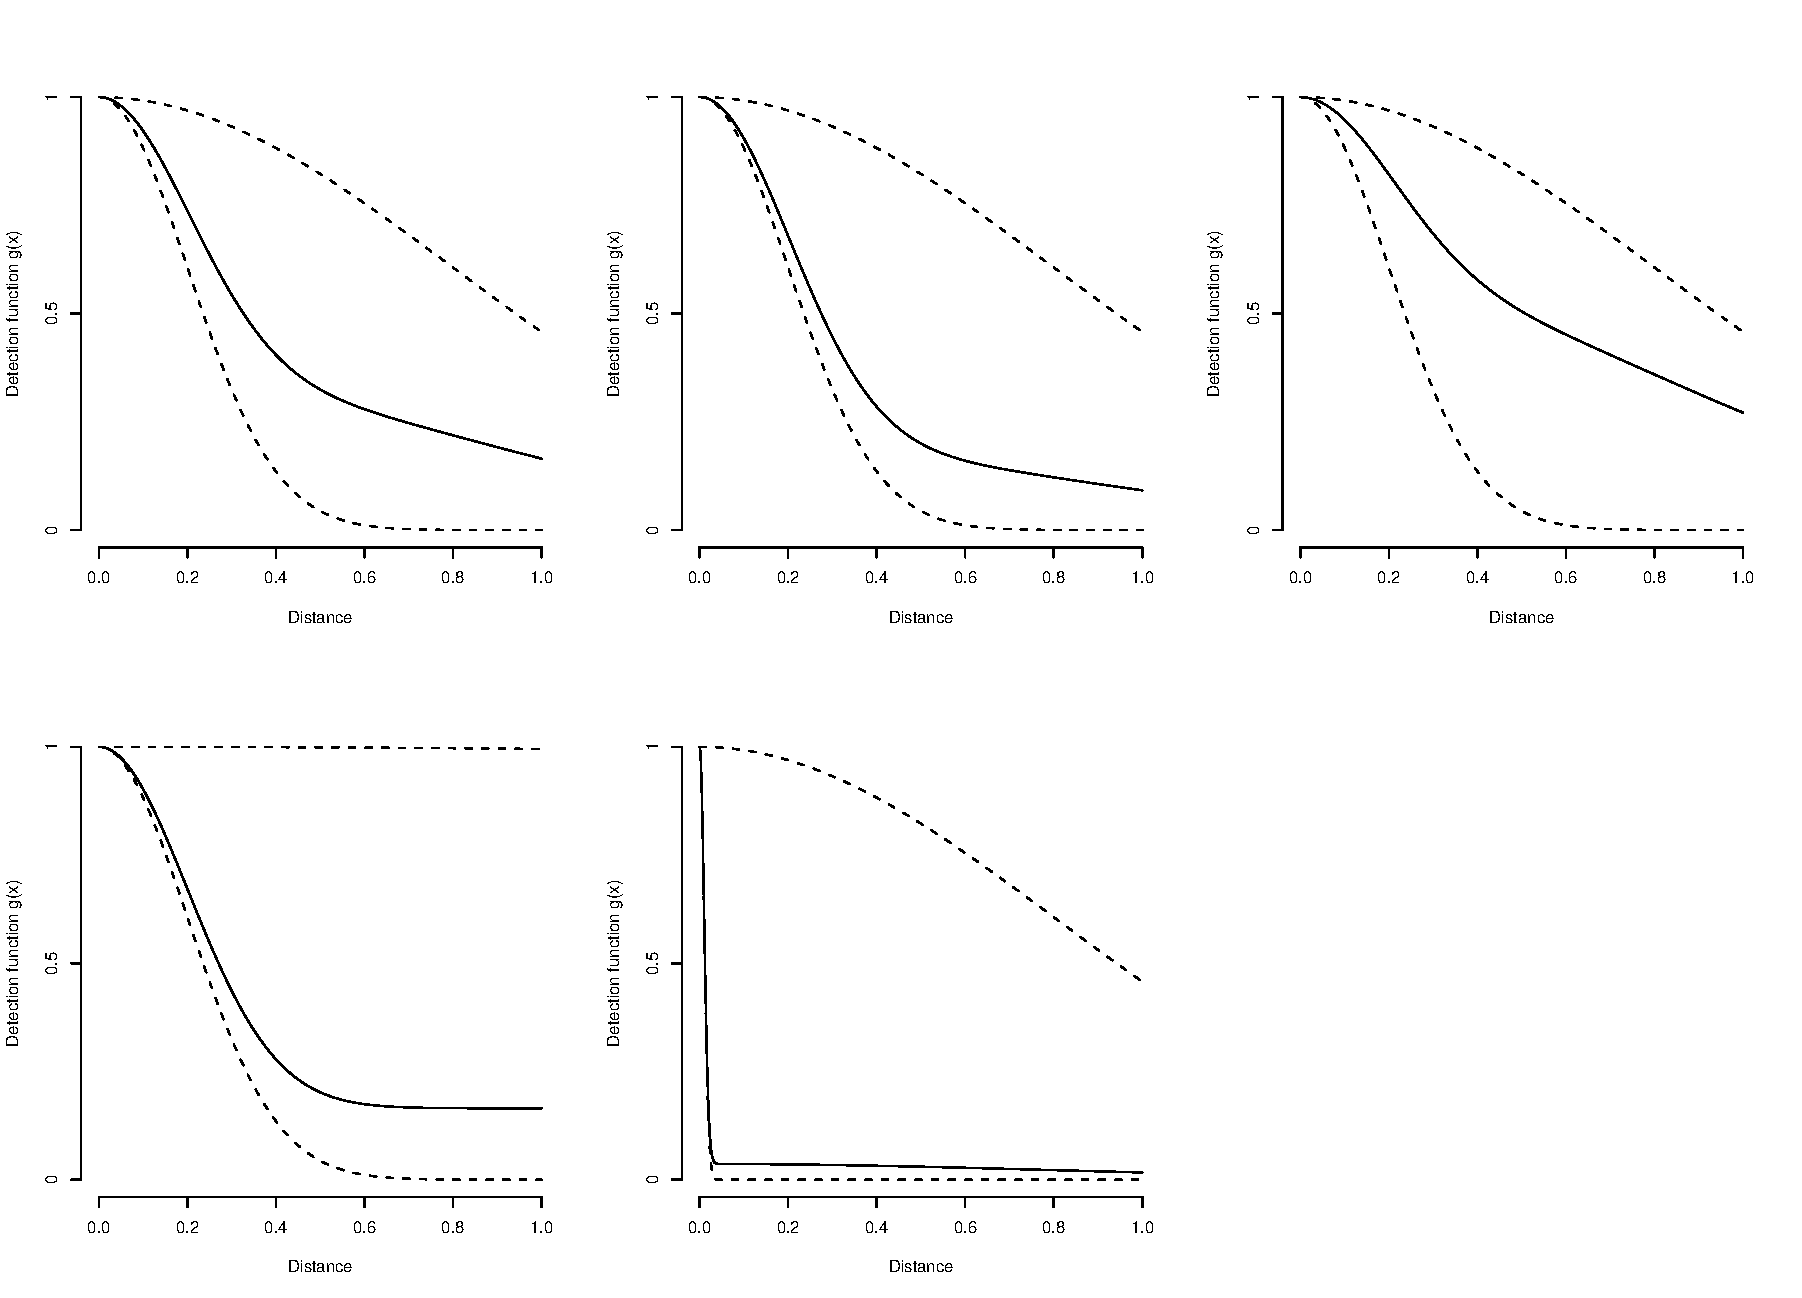
\includegraphics[width=6in]{mix/figs/nocov-detfcts.pdf}
\caption{Detection functions used for the non-covariate 2-point mixture simulations for line transects.}
\label{mmds-nocov-funcs}
\end{figure}

The data was generated using the following procedure:
\begin{enumerate}
	\item For a set sample size $n$, calculate the size of samples from each part of the mixture, $n_j = n \pi_j$ for $j=1\cdots,J$i (here $J=2$).
	\item Calculate the remainder of the samples $r = n-\sum_j n_j $ (if $r>0$) and use residual (or remainder) resampling (\cite{baker1985}) to calculate the allocation of the remaining $r$ samples:
	\begin{enumerate}
		\item Calculate the residual probabilities $\pi_j^\dagger = \pi_j - n_j/n$ for $j=1,\cdots,J$.
		\item Generate $r$ multinomial deviates with probabilities $\pi_j^\dagger$.
		\item Add these to the $n_j$s as appropriate.
	\end{enumerate}
	\item Generate $n_j$ deviates from a truncated normal distribution (truncation set to $w$, which is $1$ here), with the corresponding $\sigma_j$ as it's scale parameter and mean zero.
	\item Calculate the true abundance via the Horvitz-Thompson-like estimator $N=n/p$.
\end{enumerate}
Note that we do not have to generate from a half-normal distribution, since we can simply take the absolute value of the truncated normal deviates. This is implemented in \texttt{sim.mix.nocov()} function in \texttt{mmds}.

Figure \ref{mmds-nocov-boxplots} shows boxplots of the differences parameter estimates  and the true parameters on the $\beta$ and $\alpha$ scale (the columns of the plot). Each row corresponds to one of the scenarios in table \ref{mmds-nocov-simtable} and the colour indicates the optimisation method used. Overall we can see a nice pattern of decreasing variability and convergence towards zero as the sample size increases.

% big boxplots of par estimates
\begin{figure}[hp]
\centering
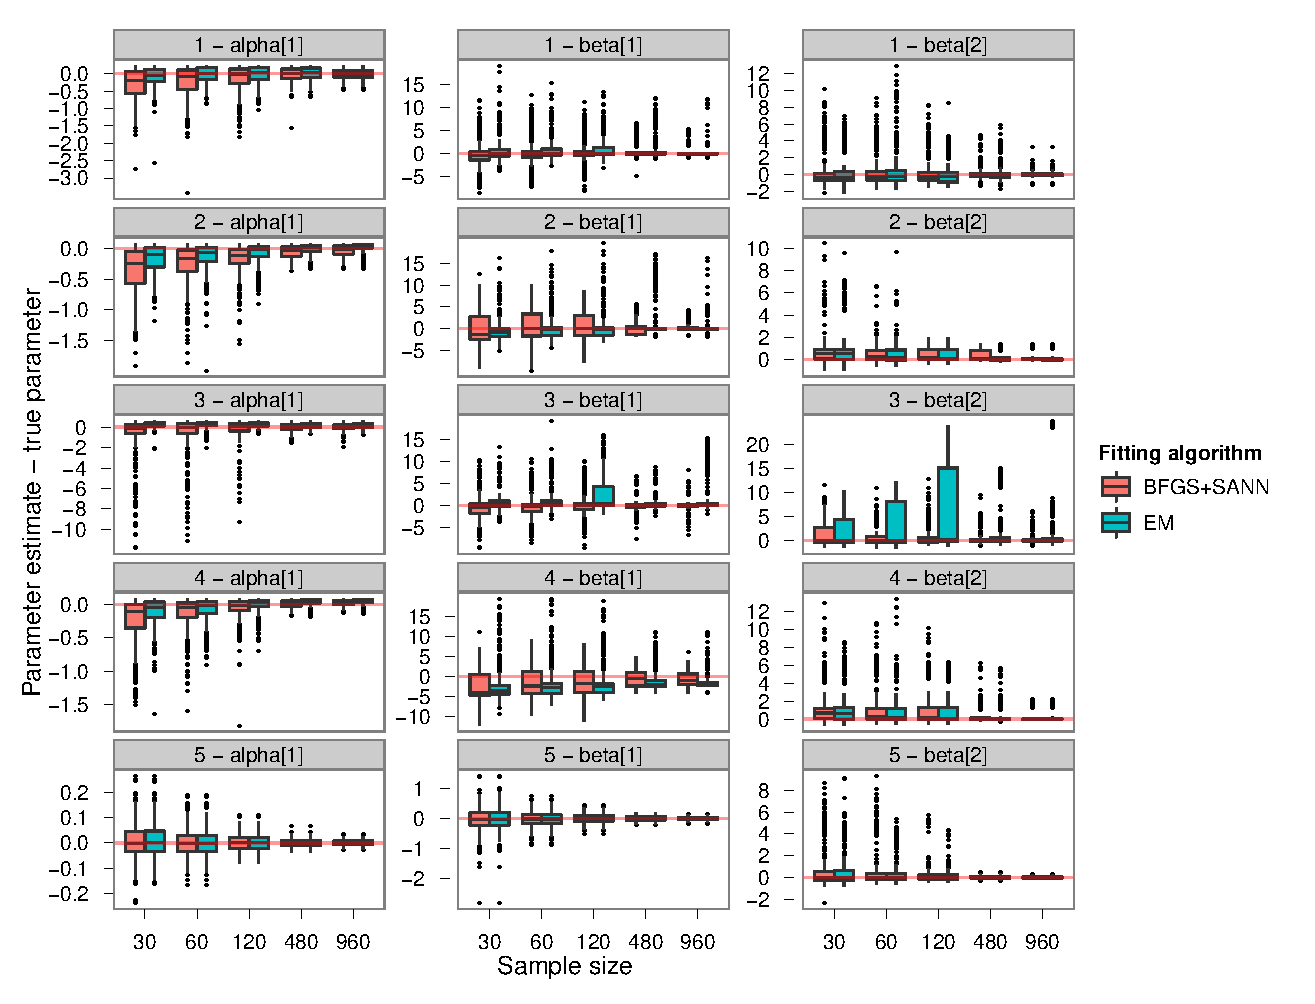
\includegraphics[width=7in]{mix/figs/nocov-boxplots.pdf}
\caption{Boxplots of difference between estimated and true parameter for the non-covariate line transect simulations. Rows correspond to the simulation numbers given in \ref{mmds-nocov-simtable}, columns correspond to parameters. Colours encode the fitting algorithm used.}
\label{mmds-nocov-boxplots}
\end{figure}
% generated by mmds/paper/papersims/nocov/analyse.R

Figure \ref{mmds-nocov-N-boxplots} also shows a reduction in variability and convergence toward zero as sample size increases. In these plots the differences between estimated and true abundance are rescaled by the true abundance since at larger sample sizes the true population is larger and they must be adjusted (see the final step in the data generation procedure, above). Table \ref{mmds-nocov-N-boxplots} shows the bias in the estimates of abundance. 

% boxplots of N
\begin{figure}
\centering
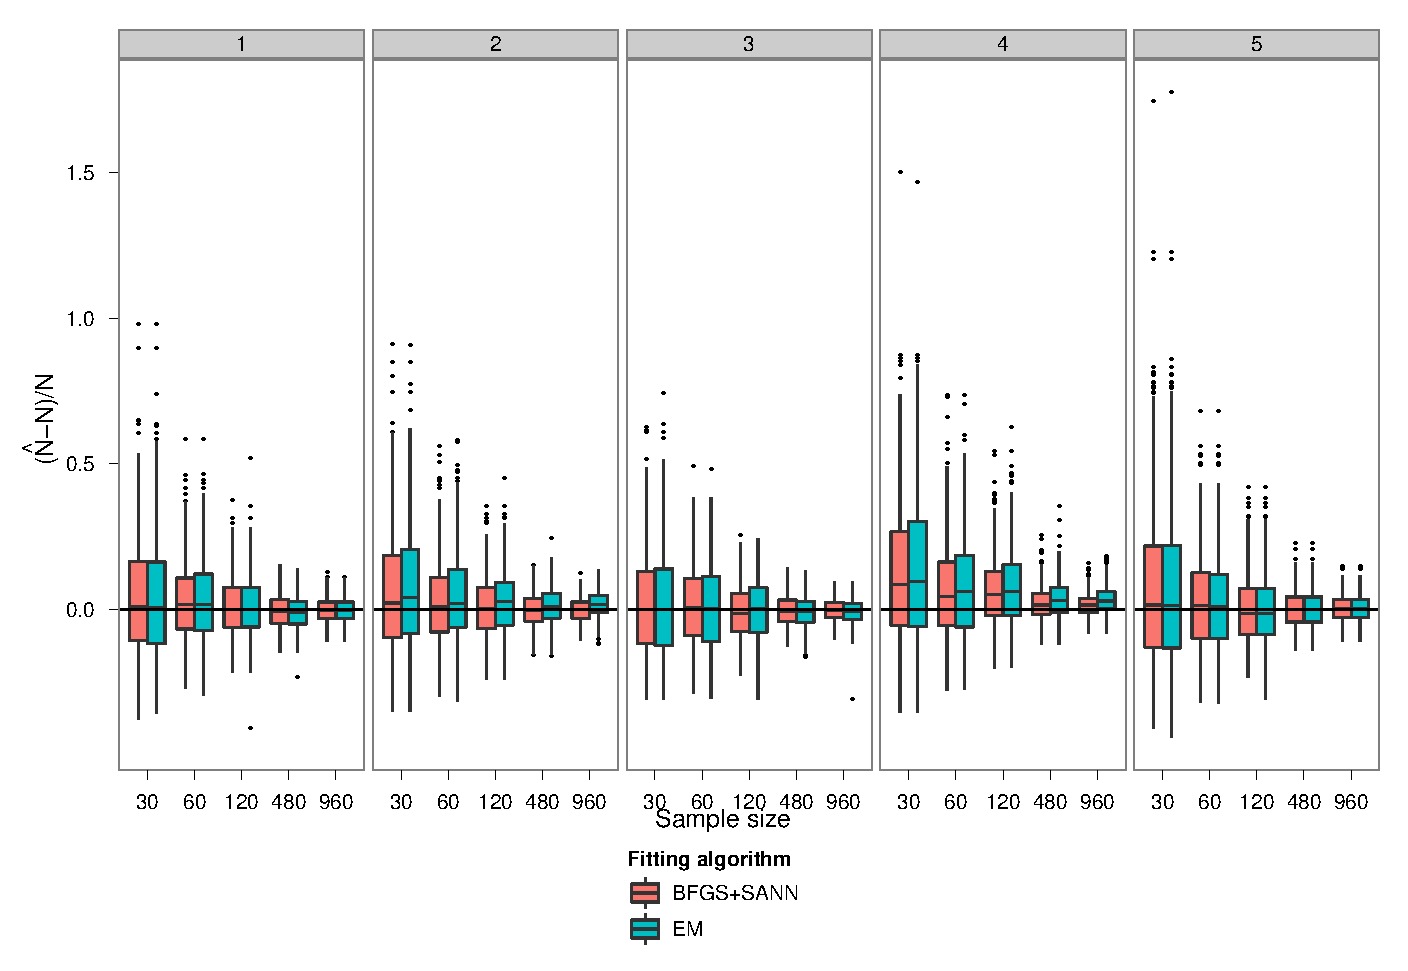
\includegraphics[width=6in]{mix/figs/nocov-N.pdf}
\caption{Boxplots of the difference between estimated abundance and true abundance divided by true abundance for each of the non-covariate line transect simulations with colour-coded fitting method. Division by the true abundance rescales to take into account at larger sample sizes the true population size is larger.}
\label{mmds-nocov-N-boxplots}
\end{figure}
% generated by mmds/paper/papersims/nocov/N-analyse.R

%\begin{sidewaystable}[ht]
\begin{table}[ht]
\begin{tabular}{c || c c | c c | c c | c c | c c}\\
Sample size & \multicolumn{2}{c |}{30} & \multicolumn{2}{c |}{60} & \multicolumn{2}{c |}{120} & \multicolumn{2}{c |}{480} & \multicolumn{2}{c}{960}\\ 
%Simulation & BFGS+SANN & EM & BFGS+SANN & EM & BFGS+SANN & EM & BFGS+SANN & EM & BFGS+SANN & EM\\
& BFGS &  & BFGS &  & BFGS &  & BFGS &  & BFGS & \\
Simulation & +SANN & EM & +SANN & EM & +SANN & EM & +SANN & EM & +SANN & EM\\
\hline
\hline
1 & -2.02  & -2.055  & -1.539  & -1.483  & -0.984  & -1.172  & 3.989  & 6.377  & 2.647  & 2.501\\
2 & -2.777  & -3.595  & -3.627  & -5.941  & -1.304  & -5.884  & 2.334  & -11.115  & -0.249  & -32.08\\
3 & -1.414  & -1.265  & -0.96  & 0.192  & -0.294  & 9.266  & 4.562  & 13.858  & -0.058  & 36.264\\
4 & -4.929  & -5.423  & -7.237  & -8.753  & -10.029  & -12.629  & -16.262  & -25.028  & -29.387  & -51.107\\
5 & -2.207  & -2.16  & -1.538  & -1.514  & -0.382  & -0.382  & 0.831  & 0.831  & -1.064  & -1.064
\end{tabular}
\label{mmds-nocov-N-boxplots}
\caption{Bias in estimates of $\hat{N}$ for the non-covariate 2-point line transect simulations.}
% generated by /mmds/paper/papersims/nocov/N-table.R 
%\end{sidewaystable}
\end{table}




\subsubsection{Non-covariate 3-point mixtures for line transect data}

Two scenarios were used to test 3-point mixtures. The parameters are given in table \ref{mmds-3pt-simtable} and the corresponding detection functions are given in figure \ref{mmds-3pt-funcs}. Data was generated using the same process as for the 2-point mixtures but with $J$ set to $3$.

As well as fitting 3-point mixture models to the data, 2-point models were also fit. This was to investigate the flexibility 2-point mixtures.

% Table of parameters
\begin{table}[h]
\centering
\begin{tabular}{c c c c c c}
Sim no. & $\beta_{10}$ & $\beta_{20}$ & $\beta_1$ & $\pi_1$ & $\pi_2$\\
\hline
\hline
1 & -0.22 & -0.69 & -2.30 & 1/3 & 1/3 \\ 
2 &  2.71 & -1.39 & -3 & 0.1 & 0.4 \\
\end{tabular}
\label{mmds-3pt-simtable}
\caption{Parameters used in the 3-point line transect simulations.}
\end{table}

% detection functions for 3point
\begin{figure}
\centering
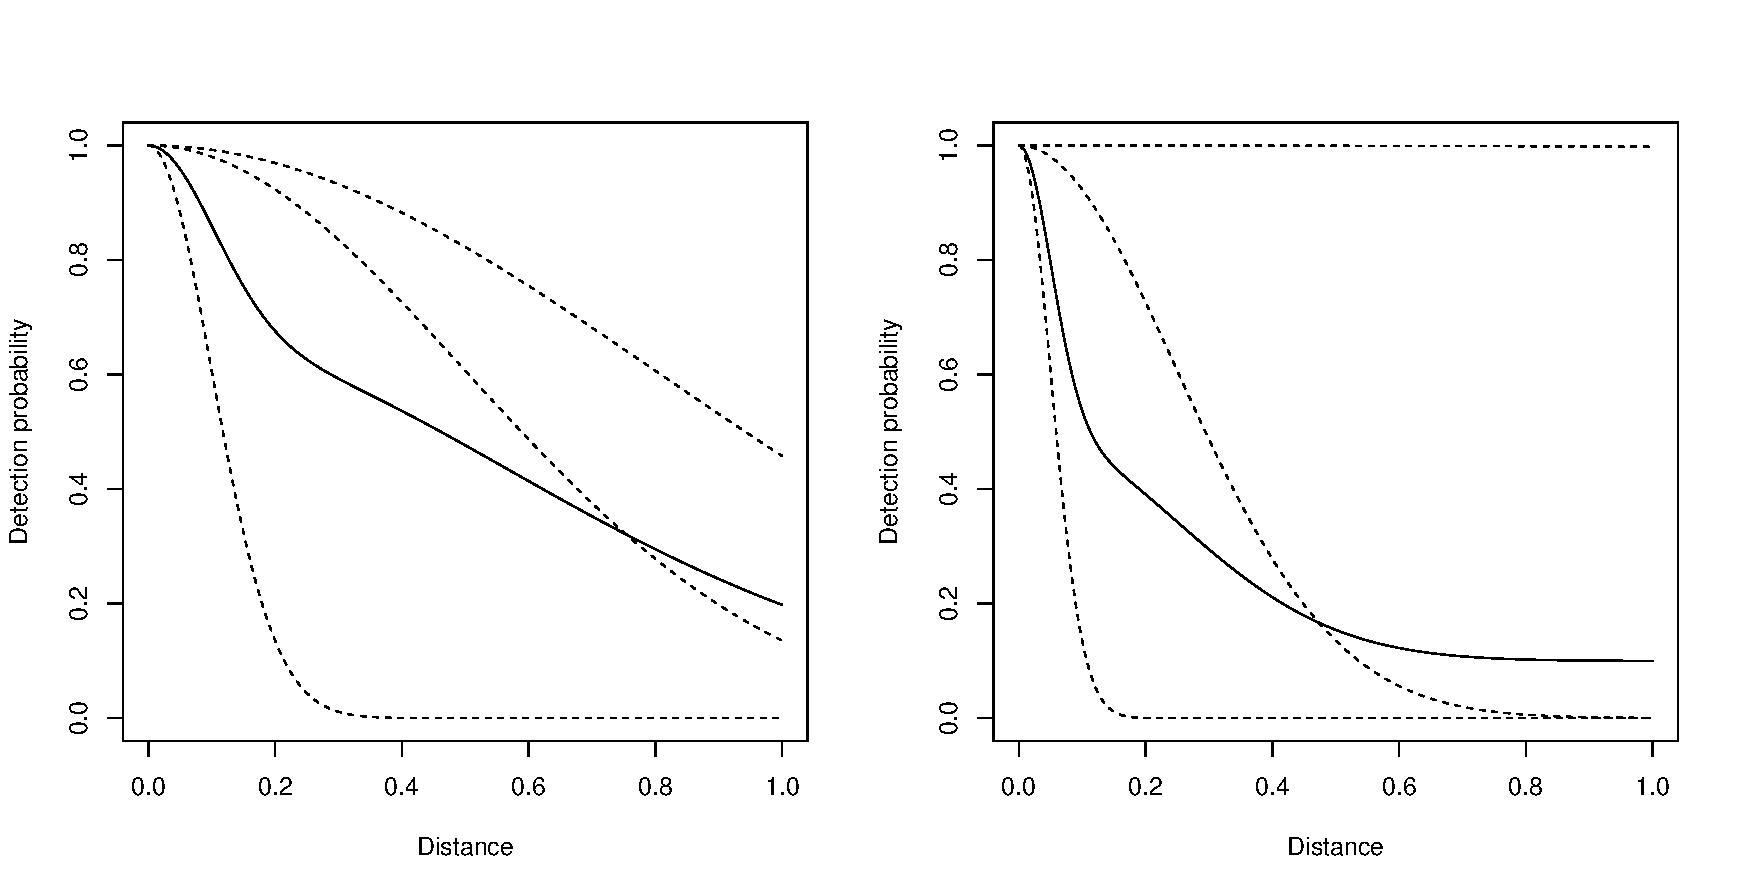
\includegraphics[width=6in]{mix/figs/3pt-detfcts.pdf}
\caption{Detection functions used for the non-covariate 3-point mixture simulations for line transects.}
\label{mmds-3pt-funcs}
\end{figure}

Figure BLAH shows the boxplots of the differences between the parameter estimates and the true parameters for when the 3-point mixtures were fit to the 3-point data.

For the 2-point fits, we can only compare the estimates of $\hat{N}$. These are shown along with the boxplots for the 3-point models in figure BLAH



\subsubsection{Covariate 2-point mixtures for line transect data}

Two models were used to test covariate 2-point mixtures for line transect data. In both cases the models had scale parameters obeying:
\begin{equation}
\sigma_{i1} = \exp(\beta_{10}+z_{i1} \beta_1),
\sigma_{i2} = \exp(\beta_{20}+z_{i1} \beta_1).
\label{mmds-test-covar-formula}
\end{equation}
In one model $z_{i1}$ was a dichotomous factor variable and in the other $z_{i1}$ was a continuous variable. In the dichotomous case, half of the observations were assigned to level 0 of the covariate and half to level 1. In the continuous case, covariates were taken to be $n$ equally spaced evaluations of the CDF of a standard normal distribution from -4 to 4. Fixed covariate values were used to minimize the complexity of the models and to check that the models would fit in the simplest scenarios TKTKTK more justification here

The data generation process was similar to that of the non-covariate line transect models:
\begin{enumerate}
   \item Generate a set of covariate values $z_{ik}$ for $i=1,\cdots,n$ and $k=1,\cdots,K$ (here $K=1$). 
	\item For a set sample size $n$, generate a set of $n$ multinomial random deviates, with probabilities $\pi_j$ for $j=1,\ldots J$. These are the mixture parts that the observations will belong to.
   \item Calculate the parameter for each of the observations using the formula in (\ref{mmds-test-covar-formula}), the mixture-appropriate parameters and the corresponding covariate values.
	\item Generate $n$ deviates from a truncated normal distribution, with the corresponding $\sigma_j(z_{ik})$ as it's scale parameter and mean zero.
	\item Calculate the true abundance via the Horvitz-Thompson-like estimator $N=\sum_{i=1}^n \frac{1}{P_a(z_i)}$.
\end{enumerate}

The parameters used to generate the data for the two scenarios are shown in table \ref{mmds-cov-simtable}. Plots of the detection functions are shown in figures \ref{mmds-cov1-detfct} and \ref{mmds-cov2-detfct}. Plots of the average detection function, the quantile/factor levels (averaged over mixtures) and mixture parts (averaged over covariate levels/values) are shown.

% Table of parameters
\begin{table}[ht]
\centering
\begin{tabular}{c c c c c}
Sim no. & $\beta_{10}$ & $\beta_{20}$ & $\beta_1$ & $\pi_1$\\
\hline
\hline
1 & -2.30 & -0.29 & -0.51 & 0.4\\
2 & -1.61 & -0.22 & -0.92 & 0.4 \\
\end{tabular}
\label{mmds-cov-simtable}
\caption{Parameters used for the 2-point covariate line transect simulations.}
\end{table}

\begin{figure}
\centering
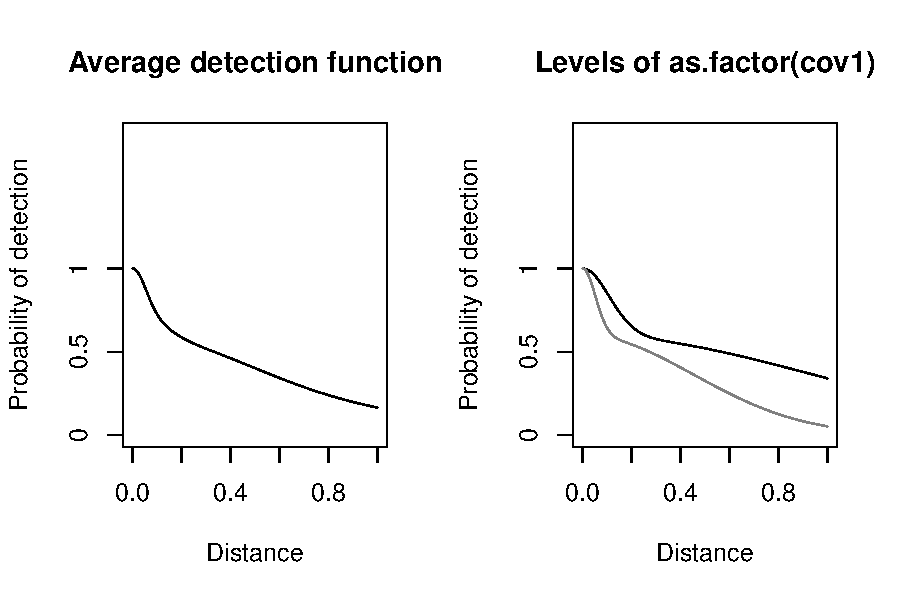
\includegraphics[width=6in]{mix/figs/covsim1-detfct.pdf}
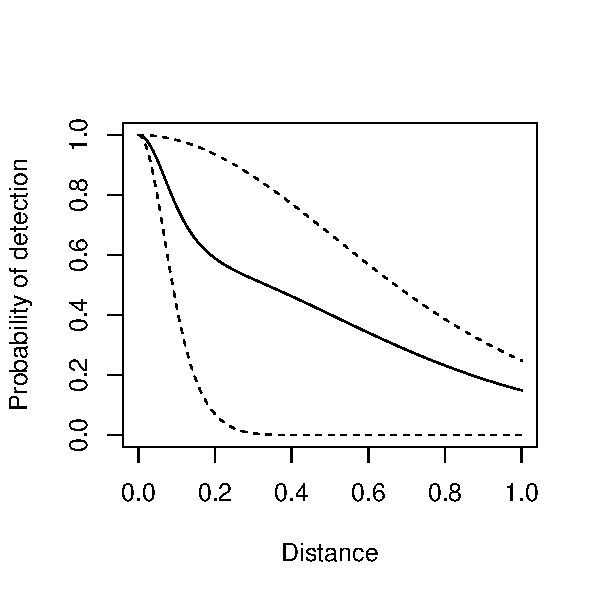
\includegraphics[width=4in]{mix/figs/covsim1-detfct-comp.pdf}
\caption{Detection function plots for the first scenario for the covariate mixtures. Top left shows the detection function averaged over both (observed) levels of the covariate and the mixture parts and top right shows the two levels of the covariate averaged over the mixture parts. The bottom plot shows the per-mixture part detection function averaged over the covariate levels.}
\label{mmds-cov1-detfct}
\end{figure}
% generated by mmds/paper/papersims/cov/plotcov.R

\begin{figure}
\centering
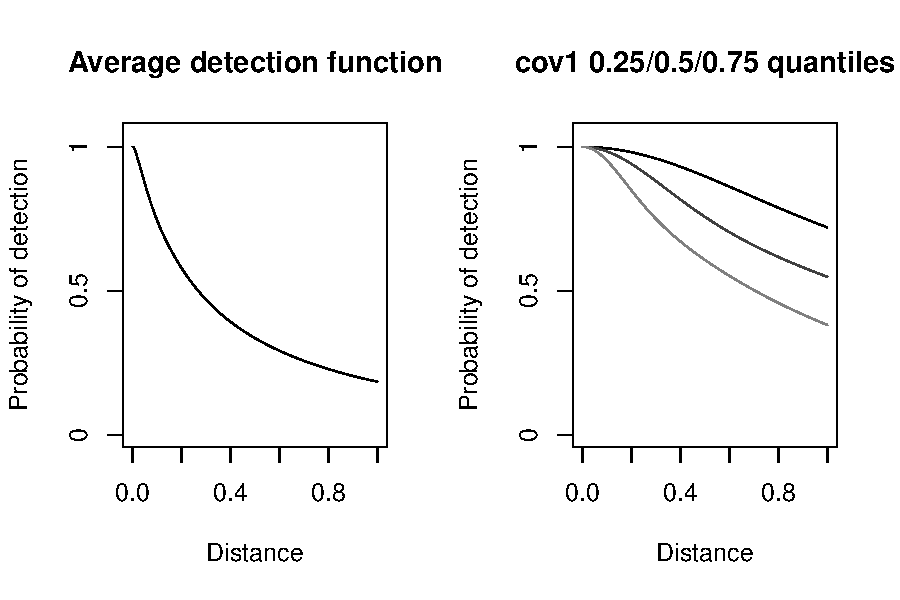
\includegraphics[width=6in]{mix/figs/covsim2-detfct.pdf}
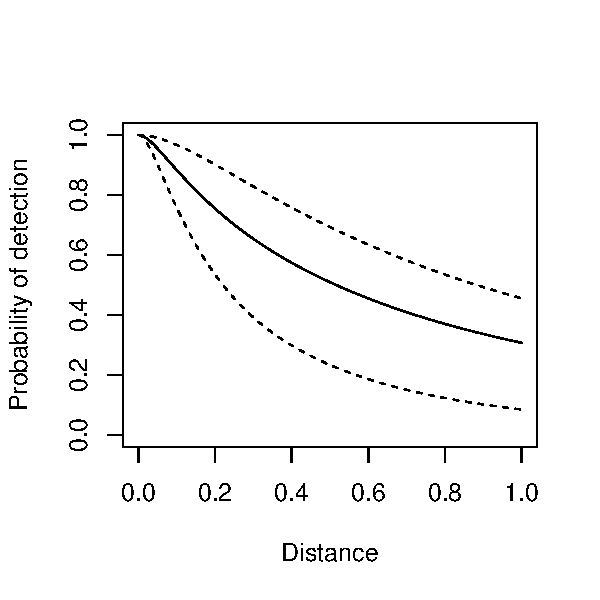
\includegraphics[width=4in]{mix/figs/covsim2-detfct-comp.pdf}
\caption{Detection function plots for the second scenario for the covariate mixtures. Top left shows the detection function averaged over all of the observed covariate values and the mixture parts and top right shows the 25\%, 50\% and 75\% quantiles of the observed covariate values averaged over the mixture parts. The bottom plot shows the per-mixture part detection function averaged over the observed covariates.}
\label{mmds-cov2-detfct}
\end{figure}
% generated by mmds/paper/papersims/cov/plotcov.R

As well as fitting the ``correct'' model to the data, a 3-point model with no covariates was also fit to the data, to see what effect misspecifying the model would have on the results. As with the 3-point models above when a 2-point model was fit to the data, we cannot compare the parameters directly, we must instead compare the estimates of the abundance.

% Plots of parameter results.
\begin{sidewaysfigure}
\centering
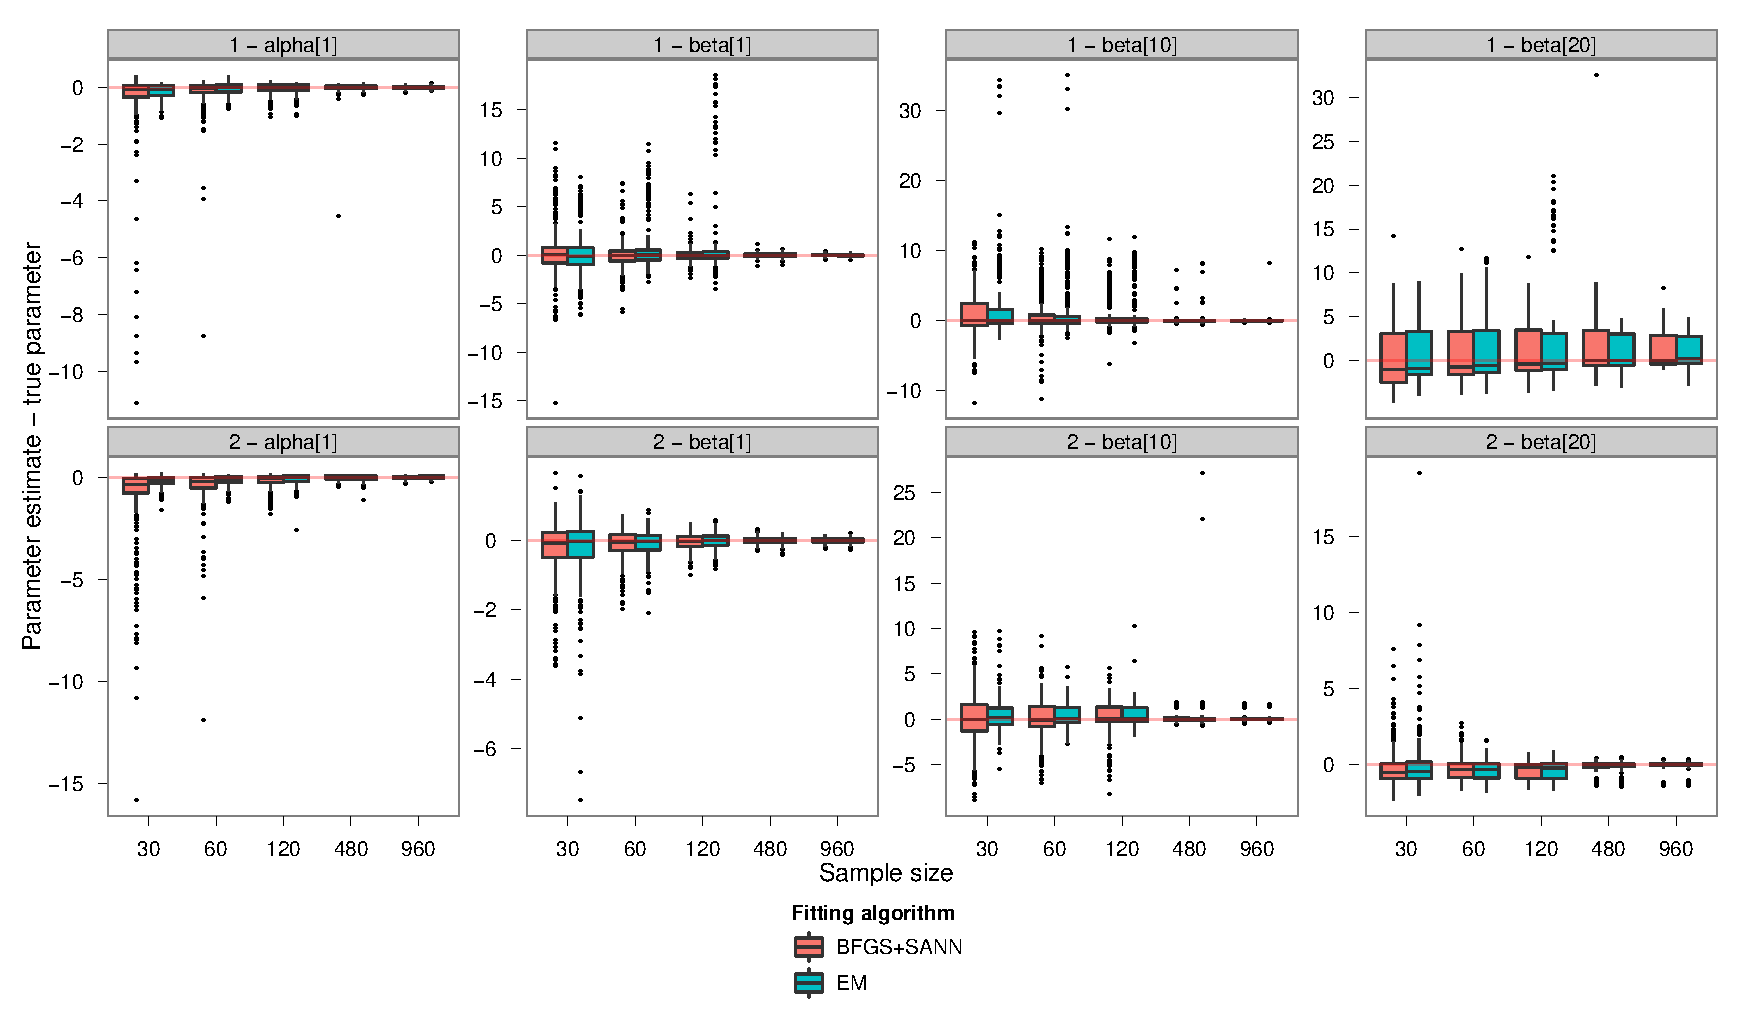
\includegraphics[width=6.84in]{mix/figs/cov-boxplots.pdf}
\caption{Boxplots of the differences between the true parameter values and the estimated parameter values for the covariate simulations. Columns correspond to parameters, rows to simulation scenarios.}
\label{mmds-cov-boxplots}
\end{sidewaysfigure}
% generated by mmds/paper/papersims/cov/analyse.R

% Plots of abundance results.
\begin{figure}
\centering
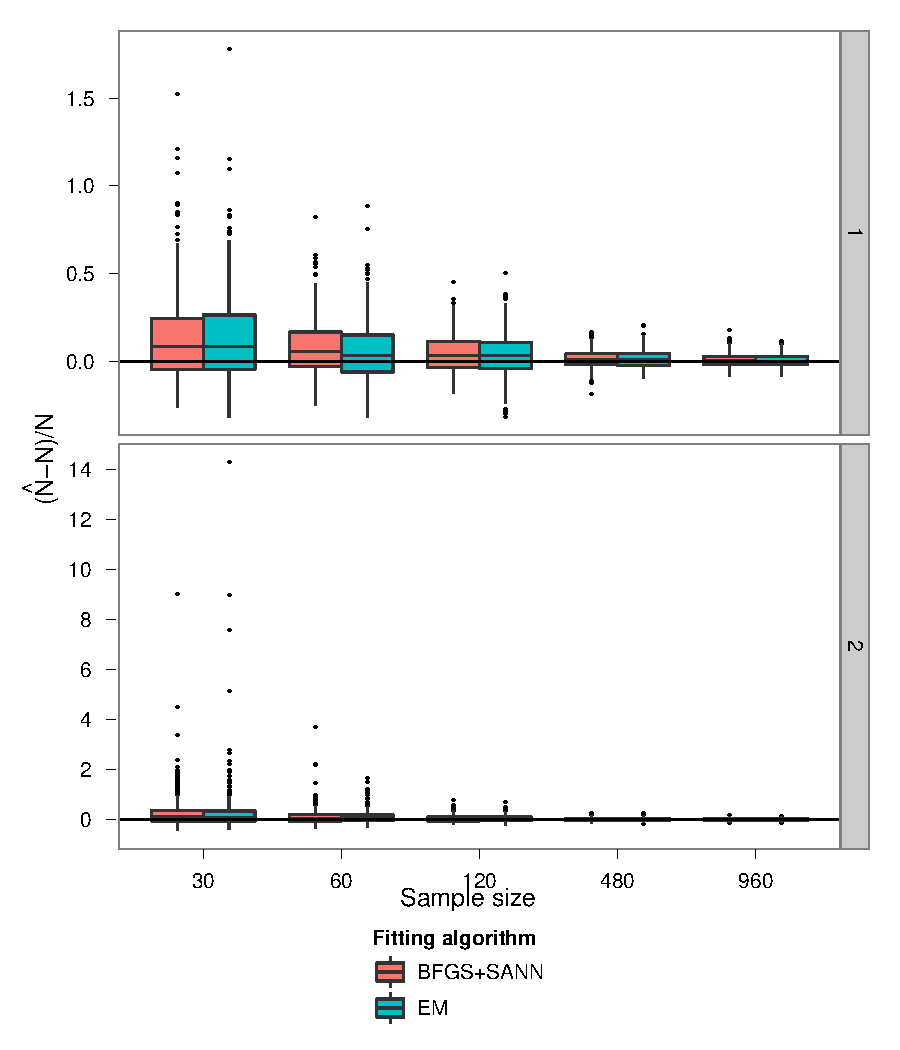
\includegraphics[width=6in]{mix/figs/cov-N.pdf}
\caption{Differences between the estimated and true abundances for the covariate simulations, rescaled by the true abundances. Left column shows when a model with the same form as the model the data was generated from was used, the right column when a 3-point mixture was fit to the data.}
\label{mmds-cov-N-boxplots}
\end{figure}
% generated by mmds/paper/papersims/cov/N-analyse.R

Figure \ref{mmds-cov-boxplots} shows boxplots of the differences between the true parameters and the estimates given by fitting a covariate moel to the data with the correct formula. Again we see a rather nice convergence toward the true value (ie. zero in the plots).

Looking at the scaled differences between the true abundance and the estimates given for both the covariate and 3-point models in figure \ref{mmds-cov-N-boxplots}, we can see that there is again a good convergence towards the truth with increasing sample size, except in one case. In the second scenario (continuous covariate) when a 3-point mixture is fitted we see only a reduction in variability and no y



\subsubsection{Non-covariate 2-point mixtures for point transect data}



\subsection{Real data}

Just source in the .tex from the vignette?

Probably not.


%%%%%%%%%%%%%%%%%%%%%%%%%%%%%%%%%%%%%%%%%%%%%%%%%%%
\section{Conclusion}


%\section{Acknowledgements}
%
%I would like to thank David Borchers for his comments on my MMath thesis, on which this work was based, as well as the parametrisation for the mixture proportions. I would also like to thank Jeff Laake and Steve Buckland for interesting discussions about the topic. Finally I would like to thank Len Thomas my co-author.
%
%Outline of the EM algorithm is taken from the very helpful set of notes by \cite{piater}.

